\documentclass[conference]{IEEEtran}
\IEEEoverridecommandlockouts
% The preceding line is only needed to identify funding in the first footnote. If that is unneeded, please comment it out.
\usepackage[T1]{fontenc}
\usepackage[utf8]{inputenc}
\usepackage[spanish]{babel}	
\usepackage{amsmath,amssymb,amsfonts}
\usepackage{cite}
%\usepackage{algorithmic}
\usepackage{graphicx}
\usepackage{textcomp}
\def\BibTeX{{\rm B\kern-.05em{\sc i\kern-.025em b}\kern-.08em
    T\kern-.1667em\lower.7ex\hbox{E}\kern-.125emX}}
\begin{document}

\title{Modelo de Programación MapReduce para Hadoop}

\author{\IEEEauthorblockN{1\textsuperscript{st} Francisco Sans}
\IEEEauthorblockA{\textit{Centro de Comptuación Gráfica} \\
\textit{Universidad Central de Venezuela}\\
Caracas, Venezuela \\
francisco.sans@ciens.ucv.ve}
}

\maketitle

\begin{abstract}
El volumen de datos producidos que deben ser almacenados y procesados a aumentado de manera considerable en los últimos tiempos.
Además, recientemente ha surgido la necesidad de poder analizarlos y obtener información significativa a partir de estos datos.
Por ello, han surgido herramientas como Hadoop, las cuales de manera eficiente permiten almacenar y realizar operaciones sobre grandes cantidades de datos.
Uno de los aspectos más relevantes de esta herramienta es el uso del modelo de programación MapReduce, el cual permite el procesamiento eficiente de los datos.
Este trabajo tiene como objetivo servir como una introducción teórica a este modelo de programación y su uso en Hadoop.
\end{abstract}



\begin{IEEEkeywords}
Haddop, MapReduce, Modelo de Programación
\end{IEEEkeywords}



\section{Introduction}
\label{intro}

Actualmente se produce de manera diaria grandes volúmenes de datos que sobrepasan las capacidades de almacenamiento y de procesamiento de una computadora convencional~\cite{Holmes12}.
Recientemente, el campo de estudio de \textit{big data} trata de solventar los problemas de cómo almacenar y trabajar con volúmenes de datos excesivamente grandes, además de buscar soluciones de como analizarlos y obtener información significativa a partir de ellos.


Hadoop~\cite{Hadoop} es un sistema distribuido construido con un sistema de archivo distribuido (HDFS~\cite{HDFS10} basado en el sistema de archivos de Google GSF~\cite{GoogleFS03}), que ofrece una manera de paralelizar y ejecutar programas en grandes grupos de computadoras.


En este trabajo se hará una breve introducción al uso del modelo de programación MapReduce y su uso en Hadoop.
En la Sección~\ref{map} se expondrán los conceptos básicos de este modelo de programación.
Posteriormente, en la Sección~\ref{hadoop} se describirá como este modelo es utilizado en Hadoop.
Finalmente, la Sección~\ref{conclu} mostrará las conclusiones con algunas ideas finales acerca del tema tratado.






\cite{MapReduceII08}
\cite{BigTable08}
\cite{HDFS10}



\section{MapReduce}
\label{map}

MapReduce es un modelo de programación para procesar grandes conjuntos de datos de manera paralela masivamente~\cite{MapReduce04}.
Está inspirado en las primitivas de \texttt{map} y \texttt{reduce} presentes en Lisp y muchos otros lenguajes funcionales.
Los usuarios que utilicen un \textit{framework} MapReduce expresarán sus cálculos a realizar con solo estas dos funciones, y \textit{framework} se encargará de la paralelización y ejecución de las mismas en grandes grupos de computadoras.
De esta manera, el programador se abstrae de las complicaciones de los sistemas distribuidos. 
El rol de programador es definir las funciones \texttt{map} y \texttt{reduce}, y el \textit{framework} MapReduce se encargará de ejecutar y coordinar los códigos como se ve en la Fig.~\ref{mapreduce}.




\begin{figure*}[htbp!]
\centering
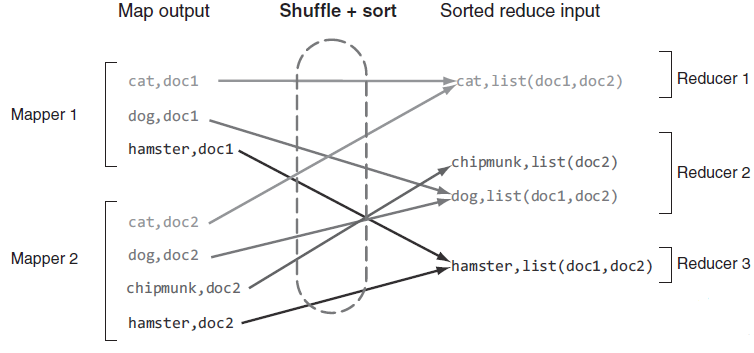
\includegraphics[width=0.8\textwidth]{images/mapreduce.png}
\caption{Etapas del \textit{framework} MapReduce. Imagen tomada de~\cite{Holmes12}.}
\label{mapreduce}
\end{figure*}


Tanto la función \texttt{map} como la función \texttt{reduce} se definen en función de pares clave/valor.
La función \texttt{map} produce pares clave/valor que luego son procesado por la función \texttt{reduce} para producir el resultado final.
La función \texttt{Map} puede definirse con respecto a sus entradas y salidas de la siguiente manera:

\begin{equation*}
map(key1, value1) \rightarrow list(key2, value2)
\end{equation*}


La función toma como entrada un par con datos en cierto dominio, que representa una entrada lógica de la fuente de datos, y es aplicada en paralelo para cada uno de los pares con clave \texttt{key1}.
Por ejemplo, en el caso de un archivo, esto podría ser una línea, o en el caso de una tabla en una base de datos, podría ser una columna. 
Como resultado, de un par de entrada se produce cero o más salidas de pares clave/valor en otro dominio diferente, y con clave \texttt{key2}.
Por ejemplo, si se quiere realizar una operación de filtro, podría producir solo las salidas que cumplen cierta condición.


Posteriormente, el \textit{framework} MapReduce se encargará de mezclar y ordenar el resultado.
Para ello, debe determinar que reductor es el encargado de recibir cada una de las salidas del \texttt{map} (proceso llamado particionamiento), y asegurar que para un reductor dado, todas las entradas se encuentra ordenadas.
El particionamiento agrupará todas las lsitas de aquellos pares que tengan la misma clave \texttt{key2}, y creará una sola lista para cada clave.


La función \texttt{reduce} es invocada una vez por cada clave única \texttt{key2} producida por el \texttt{map}, y cuyos valores están organizados en una lista.
\texttt{Reduce} función puede definirse con respecto a sus entradas y salidas de la siguiente manera:

\begin{equation*}
reduce(key2, list(value2)) \rightarrow list(key3, value3)
\end{equation*}

Cada invocación a \texttt{reduce} produce cero o más salidas con clave \texttt{key3}, aunque típicamente se produce una sola salida.
Esta salida puede ser escrita en archivos de texto en el HDFS, producir inserciones en alguna base de datos, o ser escrito en algún repositorio de datos que dependerá del trabajo que se quiera ejecutar.


%A MapReduce program is composed of a Map() procedure (method) that performs filtering and sorting (such as sorting students by first name into queues, one queue for each name) and a Reduce() method that performs a summary operation (such as counting the number of students in each queue, yielding name frequencies). The "MapReduce System" (also called "infrastructure" or "framework") orchestrates the processing by marshalling the distributed servers, running the various tasks in parallel, managing all communications and data transfers between the various parts of the system, and providing for redundancy and fault tolerance.





El \texttt{map} y \texttt{reduce} en programación funcional toma una lista clave/valor y obtiene una sola salida que combina todos los resultados obtenidos el \texttt{map}.
En contraste, en el \textit{framework} MapReduce se transforma una lista clavo/valor y se obtiene una lista de valores de resultado.


%MapReduce programs are not guaranteed to be fast. The main benefit of this programming model is to exploit the optimized shuffle operation of the platform, and only having to write the Map and Reduce parts of the program. In practice, the author of a MapReduce program however has to take the shuffle step into consideration; in particular the partition function and the amount of data written by the Map function can have a large impact on the performance and scalability. Additional modules such as the Combiner function can help to reduce the amount of data written to disk, and transmitted over the network. MapReduce applications can achieve sub-linear speedups under specific circumstances.[15]

%When designing a MapReduce algorithm, the author needs to choose a good tradeoff[10] between the computation and the communication costs. Communication cost often dominates the computation cost,[10][15] and many MapReduce implementations are designed to write all communication to distributed storage for crash recovery.


%The use of this model is beneficial only when the optimized distributed shuffle operation (which reduces network communication cost) and fault tolerance features of the MapReduce framework come into play. Optimizing the communication cost is essential to a good MapReduce algorithm



\section{MapReduce para Hadoop}
\label{hadoop}







%"Map" step: Each worker node applies the "map()" function to the local data, and writes the output to a temporary storage. A master node ensures that only one copy of redundant input data is processed.
%"Shuffle" step: Worker nodes redistribute data based on the output keys (produced by the "map()" function), such that all data belonging to one key is located on the same worker node.
%"Reduce" step: Worker nodes now process each group of output data, per key, in parallel.



%Prepare the Map() input – the "MapReduce system" designates Map processors, assigns the input key value K1 that each processor would work on, and provides that processor with all the input data associated with that key value.
%Run the user-provided Map() code – Map() is run exactly once for each K1 key value, generating output organized by key values K2.
%"Shuffle" the Map output to the Reduce processors – the MapReduce system designates Reduce processors, assigns the K2 key value each processor should work on, and provides that processor with all the Map-generated data associated with that key value.
%Run the user-provided Reduce() code – Reduce() is run exactly once for each K2 key value produced by the Map step.
%Produce the final output – the MapReduce system collects all the Reduce output, and sorts it by K2 to produce the final outcome.








%MapReduce Hadoop 

En Hadoop se tiene un motor MapReduce que corre encima del sistema de archivos (ver Fig.~\ref{motor}).
Consiste de un JobTracker, al cual los clientes suministran trabajos al MapReduce.
El JobTracker se encarga de coordinar las actividades para enviar trabajos a los nodos esclavos TaskTracker en el cluster, tratando de mantener los datos lo más cercana posible, tratando de ejecutar los trabajos en el nodo donde se encuentra la información.


\begin{figure*}[htbp!]
\centering
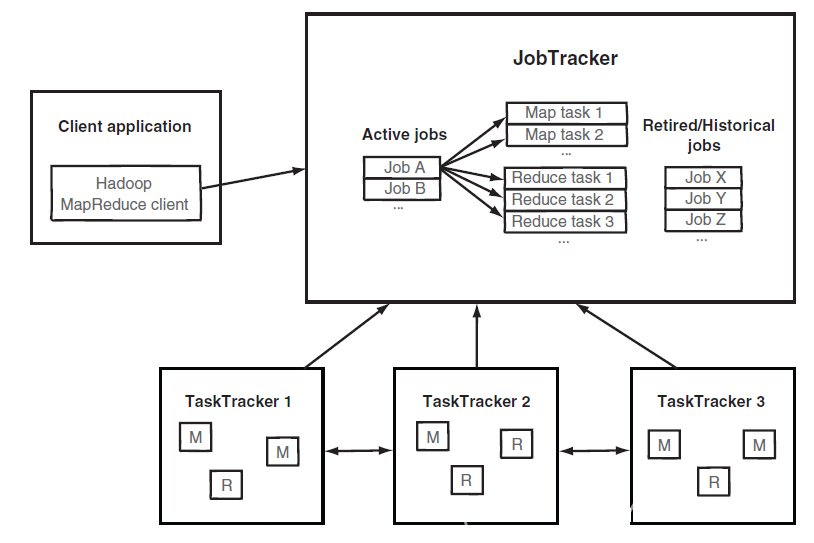
\includegraphics[width=0.8\textwidth]{images/motor.png}
\caption{Motor MapReduce de Hadoop. Imagen tomada de~\cite{Holmes12}.}
\label{motor}
\end{figure*}


Debido a que el sistema de archivos de Hadoop permite tener conocimiento de donde se encuentran los datos, el JobTracker tratará de ejecutar las tareas en el nodo que contiene la información que se necesita. 
Si esto no es posible, se seleccionará un nodo que se encuentre cercano, reduciendo el uso de tráfico de datos.
En caso de que un TaskTracker falle, el JobTracker se encargará de volver a programar el trabajo fallido.


Por otro lado, el TaskTracker es un proceso demonio que se encarga de producir procesos hijos para  ejecutar la operación \texttt{map} o \texttt{reduce}.
Típicamente, las tareas \texttt{map} leen las entradas desde el HDFS, y escriben las salidas al disco local. 
En cambio las tareas \texttt{reduce} leen las salidas del \texttt{map} desde la red y escriben sus salidas al HDFS.


Por cada proceso que el TaskTracker tenga que ejecutar, se crea una máquina virtual de Java para prevenir que un error en este proceso termine la ejecución del TaskTracker.
Cada TaskTracker tiene un número disponible de espacios.
El JobTracker asigna trabajos al espacio disponible que esté más cerca de la data.
Además, cada cierto tiempo el TaskTracker envía una señal al JobTracker para indicarle su estatus. 
Si un TaskTracker es muy lento podría retrasar todo el trabajo del MapReduce, especialmente cerca del final, donde se podría terminar esperando por la tarea más lenta.





%Cloud Dataflow
%YARN

\section{Conclusiones}
\label{conclu}



Sin embargo, MapReduce tiene ciertas desventajas al ser un modelo que no comparte información entre las ejecuciones, lo que hace que programas que necesiten sincronización global o compartir los datos sean difíciles de implementar con este modelo de programación.





%\begin{table}[htbp]
%\caption{Table Type Styles}
%\begin{center}
%\begin{tabular}{|c|c|c|c|}
%\hline
%\textbf{Table}&\multicolumn{3}{|c|}{\textbf{Table Column Head}} \\
%\cline{2-4} 
%\textbf{Head} & \textbf{\textit{Table column subhead}}& %\textbf{\textit{Subhead}}& \textbf{\textit{Subhead}} \\
%\hline
%copy& More table copy$^{\mathrm{a}}$& &  \\
%\hline
%\multicolumn{4}{l}{$^{\mathrm{a}}$Sample of a Table footnote.}
%\end{tabular}
%\label{tab1}
%\end{center}
%\end{table}



%Figure Labels: Use 8 point Times New Roman for Figure labels. Use words rather than symbols or abbreviations when writing Figure axis labels to avoid confusing the reader. As an example, write the quantity ``Magnetization'', or ``Magnetization, M'', not just ``M''. If including units in the label, present them within parentheses. Do not label axes only with units. In the example, write ``Magnetization (A/m)'' or ``Magnetization \{A[m(1)]\}'', not just ``A/m''. Do not label axes with a ratio of quantities and units. For example, write ``Temperature (K)'', not ``Temperature/K''.


\bibliographystyle{IEEEtran}
\bibliography{books}



\end{document}



